\documentclass[11pt,a4paper]{article}
\usepackage[T1]{fontenc}
\usepackage[utf8]{inputenc}
\usepackage{lmodern}
\usepackage[margin=25mm]{geometry}
\usepackage{amsmath,amssymb,amsthm,booktabs,longtable,tabularx,array}
\usepackage{graphicx,microtype,xurl}
\usepackage[round,authoryear]{natbib}
\usepackage[hidelinks]{hyperref}
\usepackage{caption,enumitem}
\captionsetup{font=small,labelfont=bf}
\setlength{\parskip}{3pt}
\setlength{\parindent}{1em}
\setlength{\emergencystretch}{3em}
\renewcommand{\arraystretch}{1.14}
\newtheorem{proposition}{Proposition}
\newcommand{\E}{\mathbb{E}}
\newcommand{\R}{\mathbb{R}}
\newcommand{\ind}{\mathbf{1}}
\newcommand{\ResultPOneMviGdp}{0.00}
\newcommand{\ResultPOneTaxGdp}{17.77}
\newcommand{\ResultPOneGiniWealth}{0.788}
\newcommand{\ResultPOneUsownershipShare}{0.00}
\newcommand{\ResultPOneMedianIncome}{1.420}
\newcommand{\ResultPOneMaxInflation}{2.04}
\newcommand{\ResultPTwoMviGdp}{19.03}
\newcommand{\ResultPTwoTaxGdp}{37.04}
\newcommand{\ResultPTwoGiniWealth}{0.754}
\newcommand{\ResultPTwoUsownershipShare}{0.00}
\newcommand{\ResultPTwoMedianIncome}{2.183}
\newcommand{\ResultPTwoMaxInflation}{2.17}
\newcommand{\ResultPFiveMviGdp}{10.57}
\newcommand{\ResultPFiveTaxGdp}{28.53}
\newcommand{\ResultPFiveGiniWealth}{0.583}
\newcommand{\ResultPFiveUsownershipShare}{29.67}
\newcommand{\ResultPFiveMedianIncome}{2.392}
\newcommand{\ResultPFiveMaxInflation}{2.12}
\newcommand{\ResultPSixMviGdp}{10.16}
\newcommand{\ResultPSixTaxGdp}{27.13}
\newcommand{\ResultPSixGiniWealth}{0.584}
\newcommand{\ResultPSixUsownershipShare}{29.67}
\newcommand{\ResultPSixMedianIncome}{2.415}
\newcommand{\ResultPSixMaxInflation}{2.13}
\newcommand{\ResultPSevenMviGdp}{5.96}
\newcommand{\ResultPSevenTaxGdp}{23.91}
\newcommand{\ResultPSevenGiniWealth}{0.560}
\newcommand{\ResultPSevenUsownershipShare}{29.67}
\newcommand{\ResultPSevenMedianIncome}{2.293}
\newcommand{\ResultPSevenMaxInflation}{2.12}
\newcommand{\SensitivityCount}{128}
\newcommand{\SensitivitySunsets}{6}
\newcommand{\SensitivityPriceBand}{128}
\newcommand{\MaxAccountingError}{6.19e-16}

\title{Bridging the AI Ownership Transition: Usownership, Programmable Money and the Limits of Seigniorage}
\author{Peplluis Esteva, Universitat de Girona}
\date{September 9, 2026}
\begin{document}
\maketitle
\vspace{-2em}
\begin{abstract}
AI-driven structural change can expand production while shifting income from labour toward automated capital. We study \emph{usownership}, a user-to-owner institution in which heterogeneous participants progressively acquire firm-specific equity according to disclosed contribution rules. The term formalises an earlier research trajectory: de la Rosa's Internet-of-Value work anticipated large-scale migration of value onto digital ledgers, while ERC-4950 (2022) explicitly introduced ``Usowners'' as NFT users who become partial owners. We embed this ownership bridge in programmable monetary infrastructure capable of coordinating granular equity allocation, vesting, dividends, settlement, and bounded monetary transfers without assuming that technology removes dilution, inflation, legal, or privacy constraints. A heterogeneous stock-flow-consistent laboratory separates ownership, targeting, taxation, and monetary instruments across 549 executed scenario paths. In the central 50-year comparison, user equity reaches 29.67\%; adding usownership to a universal-transfer benchmark lowers transfer expenditure from 19.03\% to 10.57\% of GDP, while a holding-levy architecture lowers it further to 10.16\% and conventional taxation remains 27.13\%. Matched dividend levies reproduce household cash outcomes under replication assumptions, showing that usownership's distinctive value cannot rest on relabelling redistribution. Its potential advantage instead lies in durable property rights, cumulative capital formation, participation incentives, governance, and scalable execution as assets and money become digitally programmable. We interpret 2027--2037 as an evidence-gated policy-design window and retain a 50-year horizon: if AI lowers labour's distributive role, institutions for broadening capital claims must mature before displacement outruns ownership diffusion. The paper establishes conditional mechanisms, feasibility boundaries, and a reproducible policy research agenda, not an optimal policy or post-work prediction.
\end{abstract}
\noindent\textbf{Keywords:} artificial intelligence; usownership; tokenisation; seigniorage; structural change.\\
\textbf{JEL:} E42; E62; H23; O33; P16.
\section{Introduction}
The distributional challenge of artificial intelligence is not identical to its production challenge. An economy may become better at producing goods and services while the institutions through which households obtain claims on that production change more slowly. Labour displacement is one possible source of this mismatch; it is not an inevitable implication of every AI application. Recent workplace evidence documents substantial augmentation, while models of more extensive automation admit very different long-run factor-income distributions \citep{brynjolfsson2025,acemoglu2018,trammell2026}. The policy question is how to support an uncertain transition without confusing an increase in productive capacity with an automatic improvement in household access to it.

This paper investigates \emph{contribution-weighted usownership}. The noun formalises a line of work that predates the present macroeconomic model. In 2022, the standards-track ERC-4950 proposal on entangled tokens, co-authored by Mu\~noz and de la Rosa, explicitly listed ``Usowners'' among its applications: users consuming an NFT could become partial owners of that NFT \citep{erc4950}. The present paper generalises that precursor from a paired digital-object use case to a firm-level institution and names the resulting ownership relation \emph{usownership}: \emph{user} and \emph{owner}, with \emph{-ship} denoting the durable relation. A user can progressively become an owner, with the size of the claim depending on the kind and intensity of contribution. The institution begins with predominantly private, investor-owned firms and adds recurring firm-specific equity grants to consumers, engaged users, evaluators, knowledge contributors, prosumers and co-creators. Pooling into a universal social wealth fund remains a comparator or a possible much-later institution, not an initial condition.

The ownership transition is paired with a separate income and monetary layer. Sovereign digital money and a transitional Minimum Vital Income (MVI) provide an income bridge while usownership accumulates. The conjecture is not that monetary issuance creates the real surplus distributed to users. It is that bounded seigniorage can help finance part of the lag between declining labour income and the maturity of distributed capital claims, subject to money demand, inflation and resource constraints.

Why consider this architecture rather than simply improving regulation, taxes or subsidies? An inadequate answer is that regulation changes rules, taxation changes flows and only usownership changes stocks. Property rights are themselves legal rules; a mandatory equity grant is an in-kind redistribution obligation; and taxation can finance asset grants or public investment. Moreover, a fully credible levy and rebate can reproduce the cash flows of an equity distribution. The relevant comparison is therefore between \emph{institutional implementations of redistribution}, not between legislation and its absence. Their differences concern beneficiary selection, control rights, durability, liquidity, risk, investment incentives and administrative capacity.

There is also an earlier Internet-of-Value (IoV) research precursor. De la Rosa Esteva's chapter on IoV systemic risk argued that interoperability was necessary for the democratisation of finance and property and anticipated a ``massive migration of value onto the ledgers'', described as a potential \emph{Value Deluge} whose integrity and ownership would need preservation \citep{delarosa2022iov}. That chapter did not yet contain the present contribution score, corporate dilution rule or monetary bridge. Its relevance is the architecture-level premise: value-bearing claims themselves migrate onto programmable networks, so ownership institutions can become digitally executable rather than merely digitally recorded. ERC-4950 subsequently supplied a narrower technical precursor in which linked tokens could support partial ``Usowner'' status \citep{erc4950}. The present contribution connects those earlier value and ownership primitives to structural change in production and distribution.

A second difference is becoming technologically more relevant. The prevailing financial architecture records money, securities and corporate ownership across separate account systems whose transfers require messaging, reconciliation, custodians and settlement procedures. Tokenisation instead represents money and assets as programmable claims whose ownership and transfer logic can be executed on interoperable platforms. The Bank for International Settlements describes tokenised assets as executable objects and argues that programmable platforms can bring central-bank money, commercial-bank money and financial assets into a common settlement environment \citep{bis2022,bis2023,bis2025}. The European Commission explicitly describes DLT and tokenisation as potentially paving the way towards an ``Internet of Value'' \citep{eciov2026}. This transition does not prove that blockchain is necessary or that tokenisation creates economic value by itself. It changes the implementation frontier: repeated small equity awards, vesting, dividend routing, contribution entitlements and payment can in principle be coordinated by machine-executable rules rather than reconstructed across disconnected ledgers.

This technological complement is especially important for usownership because the institution is granular and recurrent. A conventional employee stock plan may issue shares to thousands of workers; a mature digital platform could have millions of heterogeneous users whose contribution weights change continuously. If every small award requires a separate sequence of registry, custodian, payment and reconciliation events, the mechanism can be operationally prohibitive even when its economics are attractive. A programmable asset-and-money infrastructure can reduce that friction. It cannot remove the legal definition of equity, the dilution borne by existing owners, the need to verify contribution, privacy constraints or the macroeconomic incidence of seigniorage.

We make the economic comparison explicit. First, we derive a cash-flow replication result: given the same distributable profits, beneficiaries and investment response, an appropriately specified dividend levy exactly reproduces participant income from usownership without transferring legal shares. Second, we quantify the ownership-transition and financing constraints jointly. A rising aggregate user share is insufficient when displaced households do not receive grants, and increasing a holding levy eventually erodes its own monetary base. Third, we separate the contribution of equity diffusion from that of monetary redesign using matched counterfactuals rather than attributing a hybrid's whole effect to seigniorage. Fourth, we formalise how programmable monetary and asset infrastructure can reduce the operational cost of repeated ownership allocation without changing the underlying resource transfer.

The numerical laboratory has heterogeneous households, three productive activities, retained-earnings investment, an automation-linked issue rule, endogenous transaction demand and an explicit resource ceiling. It is a closed, post-reform mechanism study, not an estimated model of the European Union. The original design comprises 450 macroeconomic runs; the comparative extension adds 27 policy paths and 72 controlled robustness runs. Exact accounting identities and matched-payout tests make the exercise reproducible. Official European data provide context and units, not an empirical estimate of the behavioural parameters.

The results support a narrower, more useful proposition than unconditional superiority. In the medium-automation path, adding user equity to the universal-transfer comparator reduces year-50 MVI from 19.03\% to 10.57\% of GDP; the additional holding-levy architecture lowers it to 10.16\%. User-held equity reaches 29.67\%. Yet a targeted transfer without new equity costs 7.07\% of GDP, and a matched dividend levy generates exactly the same household cash outcomes as equity under the replication assumptions. The combined ownership and targeted-protection case reduces MVI to 1.91\% while retaining 18.75\% of GDP in residual conventional taxation. These are conditional model outcomes, not forecasts or estimates of an optimal policy.

The strongest case for usownership is therefore not that it makes fiscal policy obsolete. It is that it may institutionalise durable participant claims before and beyond a particular transfer programme, preserve a direct link between participation and the firm, and become materially easier to administer as economic value itself migrates onto programmable digital rails. Its superiority in governance, incentives and implementation cost must be established empirically. Monetary finance remains a bounded auxiliary instrument, not the source of redistributed real surplus. The analysis positions usownership as a candidate component of structural-transition policy alongside public services, competition policy, adaptive taxation and a universal protection floor.

\section{Related literature and the contribution boundary}
\subsection{Structural change: augmentation, displacement and persistent scarcity}
Task-based accounts distinguish labour-displacing automation from productivity and new-task effects \citep{acemoglu2018}. \citet{acemoglu2024} provides a restrained macroeconomic assessment, whereas \citet{trammell2026}, \citet{restrepo2025} and \citet{jones2026} consider more transformative possibilities and their limiting inputs. These are conditional theories, not alternative estimates of the same already-observed technological shock. Our declining labour-share schedule is a scenario assumption; it is not fitted to those papers or used to assert the disappearance of work.

This question also belongs to structural-change theory rather than only to monetary policy. \citet{wirkierman2023} connects demand, productivity, wages and public intervention in an empirically implemented structural accounting framework. \citet{gualerzi2026} emphasises demand and market creation in expansive structural change. The multi-sector model of \citet{dosi2022} shows that labour-market and distributive institutions can alter technological-unemployment outcomes. Our smaller laboratory does not reproduce their endogenous sectors or task dynamics; it isolates a participant-equity contract and its financing and coverage constraints.

The distinction matters empirically. \citet{brynjolfsson2025} study 5,172 customer-support agents and find a 15\% average productivity increase, with larger gains among less experienced workers. Their design does not identify economy-wide employment or wage responses. \citet{minniti2025} find heterogeneous associations between AI innovation and the labour share across European regions; patents and regional innovation are not measures of full production automation. \citet{katz2026}, in this journal, report productivity enhancement but modest observed aggregate effects during early generative-AI diffusion. This evidence motivates distributional monitoring and heterogeneous scenarios, not a forecast of an imminent post-labour economy. \citet{lamperti2026}, also in this journal, find that automation adoption is associated on average with a higher probability of inactivity in European labour-market data, with heterogeneous effects across demographic groups. At the same time, \citet{fannguyen2026} value the labour-time currently saved by observed AI usage at a labour-cost equivalent of USD~2.7 trillion, or 3.4\% of GDP; they explicitly treat that number as a valuation of time saved rather than realised GDP. Together these results strengthen the case for monitoring distributional channels while preserving uncertainty about the magnitude and timing of the macro transition.

Supply growth also depends on complementarity. Energy, compute infrastructure, chips, land and organisational capabilities can remain scarce. The simulation therefore caps potential output by a resource envelope. It does not turn the automation parameter into unlimited output, and its three activities do not constitute an input-output model of European supply chains. A useful structural-change contribution must explain both who receives productive gains and when productive constraints prevent nominal claims from becoming additional consumption.

\subsection{Taxes, insurance, industrial policy and the strongest alternatives}
The fiscal response to AI is not exhausted by a robot tax. \citet{brollo2024} discuss social protection, capital taxation and the broader fiscal response; \citet{korinek2026} analyse how transformative AI could change tax bases and the role of public capital. \citet{korinekstiglitz2026} distinguish redistribution from steering technical change. Existing capital and labour tax distortions can themselves favour excessive automation \citep{acemoglutax2020}. These contributions rule out a benchmark in which tax policy is held artificially incapable of adapting.

Optimal-tax work is particularly important as a counterargument. \citet{guerreiro2022} identify conditions for transitional robot taxation. \citet{thuemmel2023} finds that the optimal intervention can change from a subsidy to a tax and that, in the calibrated setting, most welfare gains arise through income-tax reform rather than a separate robot tax. These results do not settle the present institutional question, but they preclude claiming that an equity requirement is automatically less distortionary merely because it is not called a tax. Anticipated dilution reduces the value of an investor's future claim.

Subsidies can support learning, coordination, infrastructure and capacity rather than simply enrich current owners. \citet{juhasz2024} reviews evidence showing contextual and sometimes persistent industrial-policy effects. A subsidy can also be conditional on public or participant equity, and tax revenue can finance a social wealth fund. These are serious stock-building comparators. The present paper does not numerically optimise such an industrial-policy package; it identifies that omission rather than treating all subsidies as disposable consumption.

Cash transfers perform insurance and demand-support functions even without creating legal capital claims. Alaska's experience is informative about a permanent dividend in a market economy, not a national experiment in monetary financing of post-work incomes \citep{jonesmarinescu2020,bibler2023}. We use both targeted and universal transfers and keep their coverage differences explicit. A participation dividend cannot substitute for adequate support to a person unable to participate.

\subsection{Distributed capital, user contribution and corporate rights}
The lexical proposal in this paper has substantial conceptual ancestry. Cooperative theory explicitly identifies a ``user-owner'' principle: those who use a cooperative are also those who own and finance it \citep{dunn1988,zeuliradel2005}. Platform cooperativism later extended user and producer ownership into digital platforms; \citet{scholz2016} used the portmanteau ``produser'' for arrangements in which producer and user roles overlap, and \citet{schneider2018} analysed an ``Internet of ownership'' as an alternative to investor-only platform governance. These literatures make it inappropriate to claim that user ownership, participation-based ownership or online co-ownership originates here.

The present terminology has a more specific documented lineage. ERC-4950, created in March 2022 by Mu\~noz, de la Rosa and Easy Innova, explicitly uses the label ``Usowners'' for users who consume an NFT and become partial owners \citep{erc4950}. The proposal is a standards-track ERC whose current status is \emph{Stagnant}; it should therefore be treated as an open technical precursor, not an adopted Ethereum standard. \emph{Usownership} is the noun introduced here for the generalised institution: recurring, contribution-weighted, firm-specific equity acquisition inside firms that begin as predominantly conventional private corporations. It need not imply one-person-one-vote cooperative governance, full user financing, equal grants or immediate collective ownership. The novelty claim is consequently not that a user could become a partial owner, which ERC-4950 already stated, but that this user-to-owner relation is formalised as a scalable corporate ownership-transition mechanism and evaluated jointly with contribution measurement, dilution, income protection and monetary-financing constraints.

A bounded search conducted on 9 September 2026 also identified unrelated uses of the orthographic string \texttt{USOWNERSHIP}/\texttt{usOwnership} as a compact label for ``U.S. ownership'', including a contemporary financial-API field \citep{straitsx2026}. It did not identify an indexed source using \emph{usownership} as the noun for the generalised contribution-weighted institution defined here. The defensible lexical claim is therefore a new semantic noun in this research lineage, not ownership of an otherwise unused character string, proof of global lexical priority, or legal/trademark clearance. Search details are reported in the online supplement.

Wage-earner funds and collective capital institutions anticipated gradual ownership diffusion \citep{meidner1981,pontusson1992,furendal2024}. The AI Windfall Clause proposes advance sharing of exceptional AI gains \citep{windfall2020}. The closest contemporary fiscal antecedent is \citet{bearerfriend2025}, who propose an in-kind equity tax on generative-AI firms. Recurring grants to heterogeneous firm-specific participants differ from their one-time public-ownership instrument in incidence, beneficiaries and timing, not in the general discovery that AI equity can be redistributed.

Ownership is not merely the receipt of a labelled dividend. In incomplete-contract theory, residual control matters and its reallocation creates both benefits and distortions \citep{grossmanhart1986}. Our simulated shares give economic claims but do not endogenise voting, corporate strategy or managerial incentives. A governance advantage therefore remains a testable institutional hypothesis. Evidence from employee ownership is suggestive but not a transferable coefficient: the meta-analysis of \citet{oboyle2016} finds a small positive association with performance, not proof that user ownership raises productivity or that its dilution cost is zero.

User contributions have separate literatures. Data-as-labour proposals address compensation for data inputs \citep{dataaslabour2018}; \citet{jones2020data} study nonrival data, ownership and privacy incentives. Data Shapley provides task-specific valuation techniques \citep{ghorbani2019}; DataBright considers decentralised data ownership and rewards \citep{databright2018}. A prediction-accuracy contribution is not a universal measure of economic surplus, and a corporate share does not transfer data-processing consent. Usownership consequently needs a disclosed distributive rule, contractual boundaries and appeal procedures. It should not claim to measure each person's true marginal product merely by assigning a score.

\subsection{Monetary limits, tokenisation and the Internet of Value}
Seigniorage, inflation taxation and fiscal dominance are established subjects \citep{bailey1956,friedman1971,sargent1981,buiter2014}. Stock-flow discipline requires distinguishing issuance, cancellations, taxes, private dividends and public asset income \citep{godley2007}. Bank-created deposits are not sovereign money simply because they appear in a digital account \citep{mcleay2014}. The present sovereign-account closure excludes bank credit and legacy sovereign debt; it is deliberately not represented as a ready-made euro-area implementation.

Negative-rate proposals confront substitution into other stores of value \citep{agarwal2015}. CBDC studies analyse bank intermediation, payment efficiency and risks rather than presume that technology removes fiscal constraints \citep{auer2021,bidder2025,bindseil2025}. Circles already combines personal digital issuance and demurrage, although it is not a sovereign currency or a corporate-equity distribution system \citep{circles2026}. Neither demurrage nor digital basic income is a novelty claim here.

The implementation environment, however, is changing, and this paper also has a direct IoV precursor. De la Rosa Esteva's 2022 chapter on systemic risk in the Internet of Value argues that interoperable ledgers can support the democratisation of finance and property, analyses the fragility created by tokenised collateral and cross-ledger dependencies, and anticipates a ``massive migration of value onto the ledgers'' as a \emph{Value Deluge} requiring ownership and value-preservation mechanisms \citep{delarosa2022iov}. The chapter is conceptually relevant to the present migration-of-value premise, but it does not contain the present corporate contribution score, automation-linked issue rule or macroeconomic simulation. Those distinctions are important for a bounded novelty claim.

The term ``Internet of Value'' itself predates that chapter and this paper; Ripple was using it publicly by the middle of the 2010s and described it as an Internet on which money, securities and other assets can move as readily as information \citep{ripple2017}. The academic concept remains heterogeneous. \citet{lohmer2024} develop a definition around digital platforms, tokenisation and smart contracts, while the European Commission in 2026 explicitly described DLT and tokenisation as potentially paving the way to an Internet of Value \citep{eciov2026}. We use the expression descriptively, not as a prediction that all assets will migrate to one blockchain.

BIS work provides a more institutionally conservative formulation. Tokenisation records claims on real or financial assets on programmable platforms, integrating the asset record with rules governing transfer; programmable platforms can combine money and assets and support composability and atomic settlement \citep{bis2022,bis2023,bis2025,bis2026}. This is increasingly an operational rather than purely conceptual environment. By March 2026 the ECB reported close to EUR~4 billion of European DLT-based fixed-income issuance since 2021 and roughly EUR~1.6 billion of Eurosystem exploratory transactions across nine jurisdictions \citep{cipollone2026}. This is relevant to usownership because the proposed claim is repeated, granular and attached to corporate actions. Tokenisation can turn the right to receive, vest, transfer or distribute a participant share into an executable object. The economic claim still depends on company law, insolvency law, securities regulation and trusted information about the underlying firm.

``Programmable money'' also needs a boundary. The current digital-euro design explicitly rejects purpose-restricted money while allowing conditional payments \citep{ecbfaq2026}. Accordingly, the architecture studied here is better understood as \emph{programmable monetary infrastructure}: rules for issuance, cancellation, settlement and conditional transfer are machine-executable, but ordinary money is not restricted to a state-approved list of goods. This distinction limits both the surveillance risk and the claim of technological novelty.

\begin{table}[htbp]\centering\small
\caption{Closest mechanisms and the narrower question investigated}
\begin{tabularx}{\linewidth}{@{}p{.25\linewidth}p{.31\linewidth}X@{}}
\toprule
Literature or instrument & What is already established & Question added here \\
\midrule
Monetary finance & Income creation with money-demand and inflation constraints & How much of an ownership-transition gap fits inside that envelope?\\
Tax-transfer and robot taxes & Adaptive redistribution and transition insurance & Does equity improve anything beyond matched after-tax cash flows?\\
Industrial policy and public funds & Capacity support and publicly financed capital stocks & Can firm-specific participants acquire claims without an initial public purchase?\\
Wage-earner funds and AI equity tax & Gradual or one-off redistribution of productive claims & Recurring grants across a consumer--prosumer spectrum, initially unpooled\\
Data compensation and cooperatives & Participant value and alternative ownership institutions & Coverage, dilution, score integrity and monetary financing tested jointly\\
Internet of Value / tokenisation & Programmable assets, settlement and conditional execution & Whether granular usownership becomes cheaper to operate without changing its incidence\\
\bottomrule
\end{tabularx}
\end{table}
The contribution is an integrated comparison and a set of conditional mechanisms, not a priority claim for its individual ingredients. The review uses primary publications and official records available by 9 September 2026. Abstract-only access is recorded in the source ledger; no claims requiring unseen proofs are attributed to those sources. This is a focused, expanded review, not a database-exhaustive systematic review.

\section{Usownership: a contribution-weighted user-to-owner transition}
\subsection{The term and its institutional boundary}
We introduce \emph{usownership} as a compact noun for a specific transition in property rights, but the associated \emph{Usowner} idea has a documented precursor in the authors' earlier technical work. ERC-4950 (2022) explicitly lists ``Usowners'' as users who consume an NFT and thereby become partial owners \citep{erc4950}. The present paper takes that narrow digital-object use case and generalises it into an institution for productive firms. The semantic roots remain \emph{user} and \emph{owner}; the suffix \emph{-ship} denotes the resulting durable relation. In other words,
\[
\text{user}\;\longrightarrow\;\text{Usowner}\;\longrightarrow\;\text{usownership}.
\]
The analytical definition is: \emph{usownership is the cumulative acquisition of firm-specific ownership claims by users and other ecosystem participants according to a disclosed contribution rule}. It does not mean that every customer is automatically an equal owner, that the firm starts as a cooperative, or that a public pool owns the firm.

The lineage constrains the novelty claim. ERC-4950 demonstrates that partial user ownership and the ``Usowner'' label were already explicit in 2022; it also provides an entangled-token mechanism for linked control of a smart-contract wallet. It did not specify the present corporate dilution process, heterogeneous contribution score, automation linkage, income-coverage condition, fiscal replication benchmark or monetary transition model. Cooperative economics also has a much older user-owner principle \citep{dunn1988,zeuliradel2005}; platform cooperativism includes user-owned and ``produser-owned'' platforms \citep{scholz2016}; and \citet{schneider2018} develops an ``Internet of ownership''. A bounded search additionally found \texttt{USOWNERSHIP}/\texttt{usOwnership} as unrelated shorthand for ``U.S. ownership'' \citep{straitsx2026}. The defensible contribution is therefore the formalisation of \emph{usownership} as a generalised, contribution-weighted structural-transition institution, not the first observation that users can own digital assets. The online supplement records the search boundary.

Five properties distinguish the mechanism studied here. It is (i) \emph{gradual}, because ownership accumulates through repeated small grants; (ii) \emph{firm-specific} during the early transition rather than pooled socially; (iii) \emph{contribution-weighted}, spanning consumers, engaged users, data or knowledge contributors and prosumers; (iv) \emph{compatible with initially predominant private investor ownership}; and (v) \emph{cumulative and durable}, so successful participation can build a stock of capital rather than only a current transfer flow. These properties define the object tested below, not a claim that it dominates all tax-financed asset-building policies.

\begin{table}[htbp]\centering\small
\caption{Terminological boundary of usownership}
\begin{tabularx}{\linewidth}{@{}p{.20\linewidth}p{.28\linewidth}X@{}}
\toprule
Term/institution & Established meaning & Boundary relative to usownership \\
\midrule
User-owner principle & Cooperative users own, finance and often control the cooperative \citep{dunn1988} & Usually membership-based; does not require gradual automation-linked equity acquisition \\
ERC-4950 ``Usowner'' & NFT users can become partial owners; paired entangled tokens support linked wallet control \citep{erc4950} & Direct 2022 lexical/technical precursor; not a corporate contribution-weighted transition model \\
User-owned platform & Users collectively own or govern a digital platform & Can begin fully user-owned; usownership begins with conventional private ownership \\
Produser ownership & Producer and user roles overlap in platform cooperativism \citep{scholz2016} & Focuses producer-user duality; usownership covers a wider contribution spectrum and graded equity \\
Internet of ownership & Online ownership and governance aligned with affected stakeholders \citep{schneider2018} & Broad design agenda; usownership is a specific recurring firm-level allocation rule \\
\textbf{Usownership} & \textbf{User $\rightarrow$ owner through cumulative contribution-weighted grants} & \textbf{Gradual, firm-specific, initially unpooled and compatible with investor ownership} \\
\bottomrule
\end{tabularx}

\end{table}

\subsection{Allocation, dilution and incidence}
Let $q_{ij,t}$ be household $i$'s conventional fraction of firm $j$, $u_{ij,t}$ its usownership fraction and $\delta_{j,t}$ new participant shares relative to the pre-issue share count. With normalised contribution weights $s_{ij,t}\geq0$ summing to one for each firm,
\begin{align}
q_{ij,t}&=\frac{q_{ij,t-1}}{1+\delta_{j,t}},\\
u_{ij,t}&=\frac{u_{ij,t-1}+\delta_{j,t}s_{ij,t}}{1+\delta_{j,t}}.\label{eq:equity}
\end{align}
The second left-hand symbol is $u$, a user share, not the investment share $\nu$ used later. All pre-existing shares, including previous user grants, are diluted consistently. No equity issue creates additional machines or monetary balances in this accounting.

\begin{proposition}[Gradual ownership accumulation]\label{prop:accumulation}
Without secondary sales, and starting with no usownership, aggregate user ownership of firm $j$ is
\begin{equation}
U_{j,t}=1-\prod_{\tau=1}^{t}(1+\delta_{j,\tau})^{-1}.\label{eq:U}
\end{equation}
At constant $\delta$, this becomes $1-(1+\delta)^{-t}$, independent of how the grant pool is divided among its users.
\end{proposition}
\begin{proof}
Summing \eqref{eq:equity} over households gives $1-U_{j,t}=(1-U_{j,t-1})/(1+\delta_{j,t})$. Iteration proves the expression. Distribution among people still depends on their scores.
\end{proof}

A firm with one million pre-existing shares issuing 20,000 participant shares transfers 1.9608\% of its post-issue equity, not 2\% of the post-issue stock. If company value were unchanged at the issue, the old holders would lose that same fraction of their claim. Gradual dilution is therefore an in-kind transfer, even where legally authorised and predictable. Whether participation adds value that compensates investors is an empirical question, not an accounting consequence.

Our illustrative automation-linked schedule is
\begin{equation}
\delta_{j,t}=\bar\delta\left[\frac{a_{j,t}-a_0}{1-a_0}\right]_+,\quad
\bar\delta=0.02,\quad a_0=0.25.\label{eq:delta}
\end{equation}
The threshold delays grants until automation reaches a specified level; the cap limits the annual transfer. Both are normative scenario assumptions. Automation is difficult to measure and firms may strategically relabel technology, restructure subsidiaries or relocate rights. A deployable rule would require legal definitions, aggregation and anti-avoidance provisions that are not supplied by a blockchain.

Investment incentives cannot be assumed unaffected. If total future dividends grow at $h$ and an investor discounts at $r$, constant dilution changes a simple present-value series to $\sum_t\Pi_0[(1+h)/((1+r)(1+\delta))]^t$. The approximation raises the effective discount burden by about $\delta$. Tax relief, stronger user demand or productive contributions might offset some cost, but such offsets require evidence. The simulation consequently imposes and stresses an explicit reduced-form investment response rather than claiming incentive compatibility.

\subsection{From consumers to prosumers}
A general contribution vector can include use, meaningful engagement, feedback, data quality, knowledge, content production, compute supply, network services and governance. These are not interchangeable quantities. In the laboratory they are compressed into three synthetic dimensions: use $x$, engagement $e$ and productive creation $z$. Within each firm we apply
\begin{equation}
\widetilde s_{ij}=0.35\sqrt{\min(x_{ij},25)}+0.25e_{ij}+0.40z_{ij},\qquad
s_{ij}=\frac{\widetilde s_{ij}}{\sum_k\widetilde s_{kj}}.\label{eq:score}
\end{equation}
Use is normalised by the firm's median use; the engagement and creation inputs are bounded synthetic characteristics. The coefficients are not estimated values. They implement the proposed participation spectrum while making the distributional judgement inspectable. Consumption-only, square-root-consumption and equal-grant alternatives test sensitivity. Raw attention time is not independently rewarded.

Consider an AI platform with 10,000 users in each of six contribution classes, one million outstanding shares and a new 20,000-share pool. The following values are generated by the example code. A hypothetical EUR10 million total distribution illustrates ownership arithmetic, not a forecast of firm value or investor returns.
\begin{table}[htbp]\centering\small
\caption{Illustrative AI-platform grant: 60,000 users, six contribution classes}
\begin{tabular}{llll}
\toprule
Role & Score & New shares/person & Dividend/person (EUR) \\
\midrule
Consumer & 0.350 & 0.060 & 0.585 \\
Intensive consumer & 0.950 & 0.162 & 1.587 \\
Evaluator & 1.645 & 0.280 & 2.747 \\
Domain expert & 2.845 & 0.485 & 4.751 \\
Plugin creator & 2.995 & 0.510 & 5.002 \\
Prosumer & 2.956 & 0.504 & 4.937 \\
\bottomrule
\end{tabular}

\end{table}
The same code supplies autonomous-mobility and household-robotics examples, distinguishing ordinary users, feedback providers, infrastructure hosts, accessibility evaluators and productive contributors. A valuable user can receive more than a large spender, but the weights still embody a distributive choice. A score cannot by itself distinguish freely given feedback from compensable employment, intellectual property or data acquired without valid consent.

\subsection{Coverage, transferability and the limits of a sunset}
Let pre-transfer disposable income be $h^0_{i,t}$ and the desired income floor $z_t$. A universal top-up protecting a selected lower quantile $q$ is
\begin{equation}
h_t=\left[z_t-Q_q(h^0_{i,t})\right]_+.\label{eq:floor}
\end{equation}
This is universal payment with a quantile-based calibration, not an individual means-tested guarantee. Some people below the reference quantile can still fall short. We report that gap rather than equating a zero top-up with universal adequacy.

\begin{proposition}[A coverage condition for the income bridge]
Under \eqref{eq:floor}, the top-up is zero if and only if the selected pre-transfer income quantile reaches the floor. If a share of people larger than $q$ permanently has zero capital claims and labour income vanishes for them, a positive relative income floor cannot be replaced by aggregate usownership growth alone.
\end{proposition}
\begin{proof}
The first statement follows directly from the positive-part operator. Under the second condition the relevant income quantile approaches zero regardless of dividends received outside that group. A strictly positive floor therefore leaves a positive top-up.
\end{proof}

The distinction between a fixed real floor and one indexed to prosperity is equally important. If incomes and the floor all scale proportionately with real GDP, growth cancels from the comparison: distributional shares determine adequacy. Faster production need not shorten the bridge. In contrast, a fixed real floor becomes smaller relative to output and can disappear without equitable participation in increasing prosperity.

The baseline retains user shares; this is a strong protection assumption, not a free institutional feature. An extension allows cash-settled sales from non-wealthy holders to wealthy buyers at book value, after specified vesting. Every purchase transfers money to a seller rather than destroying it. Early sales can reconcentrate claims. Vesting, a non-transferable core or a liquid income floor can reduce that effect, but they also restrict household choice, collateral use and risk diversification. Demography, inheritance and entry of new users are not simulated; century-scale paths therefore require especially cautious interpretation.


\section{Programmable monetary architecture, incidence and accounting}
\subsection{Sovereign architecture and the boundary of the model}
The intended long-run design is sovereign programmable payment money. To obtain a tractable first model, all transaction balances are direct sovereign liabilities. Firms finance capital formation from retained earnings, and equity is owned by households. There is no endogenous bank credit, government bond market, foreign sector or asset-price equilibrium. This is a limiting monetary architecture with fully sovereign transaction balances, not a description of the current euro area or a complete narrow-banking transition proposal.

The simplification is consequential. Moving existing deposits onto sovereign accounts requires counterpart assets, bank funding arrangements, redemption rules and a plan for legacy debts. A sovereign state does not acquire the entire stock of existing broad money as spendable revenue by relabelling it. The current EU debt stock also cannot be wished away. The empirical context includes an EU debt ratio of 81.7\% in the annual 2025 first notification \citep{eurostat2026}; that liability is deliberately outside the simulated balance sheet. Thus the simulations test a conditional post-reform monetary mechanism, not the financing of the reform itself.

\subsection{Why programmable monetary infrastructure matters for usownership}
The technological claim is not that software changes the resource constraint. It is that the administrative architecture of ownership is changing as money, securities and other claims become increasingly digital and, in some settings, tokenised. The prevailing account-based paradigm typically separates identity and contribution data, company share registers, custodians, payment systems, tax records and corporate-action processing. Each institution can work well on its own, but a recurrent grant to millions of heterogeneous participants requires repeated matching and reconciliation across those systems.

An Internet-of-Value architecture changes the implementation problem by making the asset claim and some of its transfer rules machine-readable or executable. BIS work on tokenisation and unified ledgers emphasises composability and atomic settlement between money and assets rather than a requirement for permissionless cryptocurrency \citep{bis2022,bis2023,bis2025}. The European Commission similarly describes tokenisation and DLT as a possible route toward an ``Internet of Value'' \citep{eciov2026}. In that environment, a verified contribution event can update a fractional ownership claim; vesting can be enforced at the claim layer; dividends and corporate actions can follow the current holder; and a sale or voluntary diversification can settle conditionally against digital money. The same infrastructure can automate an MVI payment, a protected transaction balance, or a monetary levy and cancellation rule. It therefore provides a common execution substrate for the \emph{ownership bridge} and the \emph{income bridge}.

\begin{figure}[htbp]\centering
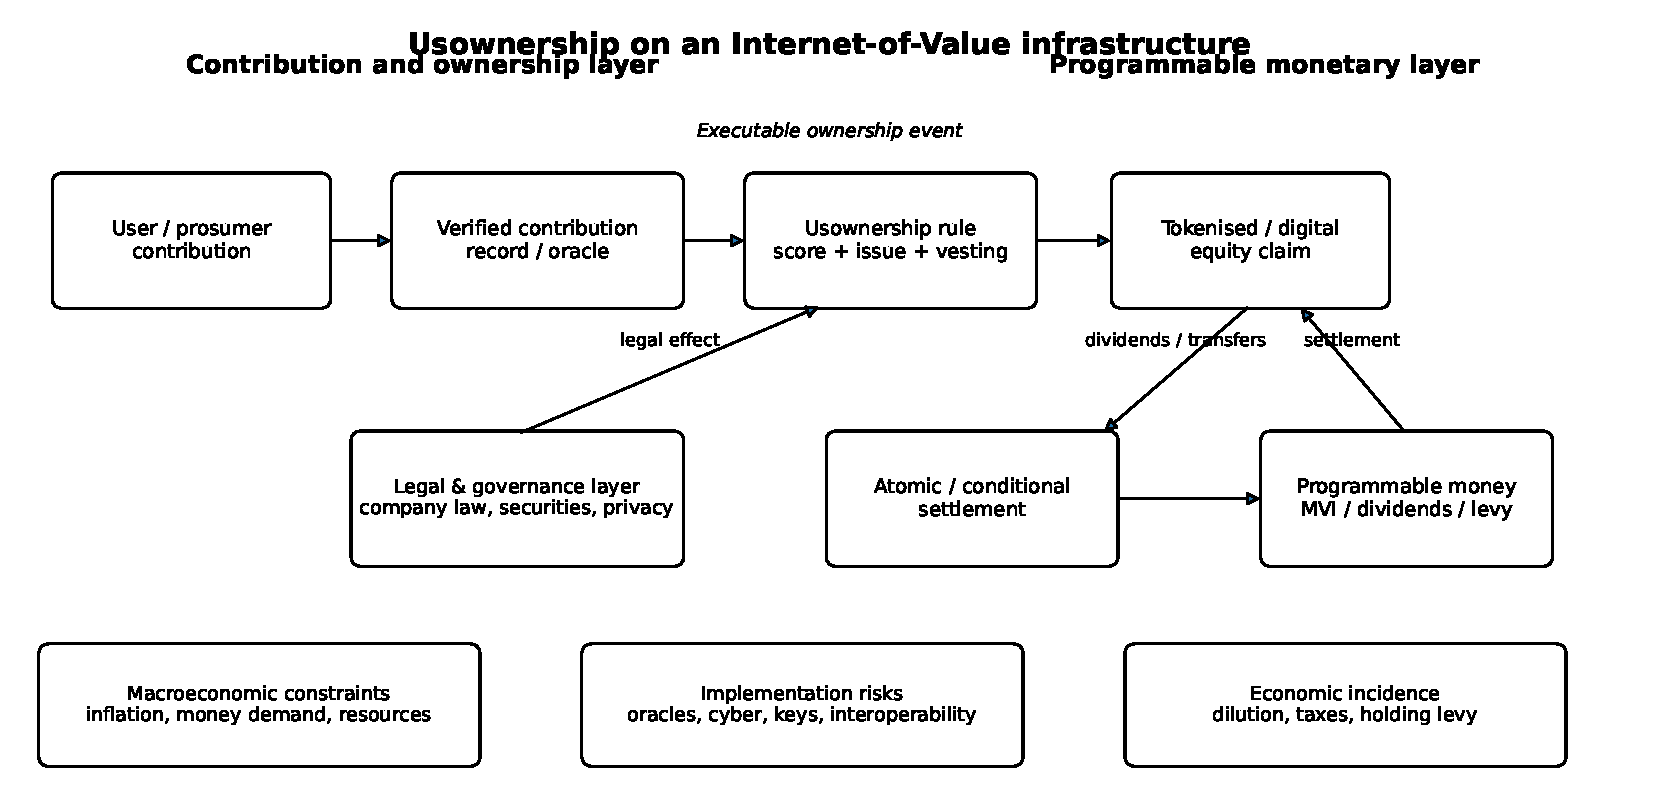
\includegraphics[width=.96\linewidth]{figures/programmable_usownership_architecture.pdf}
\caption{Usownership on programmable Internet-of-Value infrastructure. Programmability coordinates contribution evidence, equity rights and payment; legal validity, valuation, privacy and macroeconomic incidence remain outside the ledger and must be governed separately.}
\label{fig:programmable-usownership}
\end{figure}

The comparison can be stated as a measurable break-even condition rather than a technological slogan. Let $N_t$ be the number of ownership events in period $t$, $c_L$ the marginal legacy-system processing and reconciliation cost per event, $c_P$ the marginal programmable-infrastructure cost, $F_P$ its fixed operating cost, and $C_O,C_R,C_{Pr}$ the incremental costs of trustworthy contribution oracles, regulatory compliance and privacy/cybersecurity. A direct implementation advantage requires
\begin{equation}
N_t(c_L-c_P)>F_P+C_O+C_R+C_{Pr}.
\label{eq:implementation}
\end{equation}
No numerical saving is imposed in the simulation because these terms have not been empirically estimated for a national usownership regime. Equation~\eqref{eq:implementation} instead identifies the evidence required. The hypothesis becomes stronger as awards become more frequent and granular, and weaker if oracle, compliance or interoperability costs dominate the reduction in reconciliation cost.

\begin{table}[htbp]\centering\small
\caption{Implementation comparison: separate account systems and programmable value rails}
\begin{tabularx}{\linewidth}{@{}p{.22\linewidth}p{.34\linewidth}X@{}}
\toprule
Dimension & Prevailing account-based implementation & Programmable Internet-of-Value implementation \\
\midrule
Ownership record & Separate corporate/share registry and custodial records & Tokenised or digitally executable ownership claim \\
Award execution & Batch or manual reconciliation across systems & Conditional rule can update claim after verified event \\
Money/asset settlement & Payment and asset legs may use distinct infrastructures & Atomic or conditional settlement can coordinate both legs \\
Granularity & Economical for many conventional plans but micro-awards can face fixed frictions & Fractional recurrent awards can have low marginal execution cost if infrastructure is shared \\
Corporate actions & Multiple intermediaries propagate dividends, splits and transfers & Rules can propagate actions to the current claim holder \\
Policy control & Fiscal and monetary ledgers are separately administered & Issuance, protected balances, levies and burns can be auditable machine-executable rules \\
Unresolved constraints & Tax, securities, privacy, insolvency and valuation law & Same legal constraints plus oracle, cyber, key-management and interoperability risks \\
\bottomrule
\end{tabularx}

\end{table}

This framing also clarifies the word \emph{programmable}. The current digital-euro project rejects purpose-restricted ``programmable money'', while contemplating conditional payments \citep{ecbfaq2026}. Our proposal therefore concerns \emph{programmable monetary infrastructure}: rules for issuance, settlement, protected balances and cancellation can be machine-executed without restricting ordinary currency to state-approved purchases. A tokenised share is still a legal corporate claim; a smart contract cannot manufacture a valid contribution observation, determine insolvency priority by itself, or make dilution costless. Programmability is an adoption technology, not a new source of seigniorage.

Let $N_t=P_tY_t$ denote nominal GDP, $M_t$ end-of-period sovereign transaction balances, $G_t$ public purchases, $H_t$ transfers, $T_t$ conventional tax receipts and $B_t$ the monetary holding levy permanently cancelled. Define fiscal issuance before the holding levy as
\begin{equation}
F_t=G_t+H_t-T_t,\qquad M_t-M_{t-1}=F_t-B_t.\label{eq:budget}
\end{equation}
$F_t$ is a \emph{net-of-conventional-tax financing flow}, not total gross expenditure and not necessarily positive. A negative value retires currency. We report it separately from genuine net money financing $(M_t-M_{t-1})/N_t$. Counting $F_t$ and $B_t$ as independent free resources would be incorrect.

\begin{proposition}[No free monetary recycling]
Under the consolidated budget identity \eqref{eq:budget}, a currency burn can expand the expenditure financed by a given net change in money only by transferring an equal nominal amount from the balances charged. Recycling does not remove the financing incidence.
\end{proposition}
\begin{proof}
Rearranging gives $G_t+H_t=T_t+B_t+(M_t-M_{t-1})$. At a fixed net monetary change and conventional receipts, an additional unit of expenditure requires an additional unit of levy. Implementation as a fee followed by cancellation does not change the identity.
\end{proof}

With $m_t=M_t/P_t$ and $\pi_t=P_t/P_{t-1}-1$, the exact discrete decomposition is
\begin{equation}
\frac{F_t}{P_t}=m_t-m_{t-1}+\frac{\pi_t}{1+\pi_t}m_{t-1}+\frac{B_t}{P_t}.\label{eq:seign}
\end{equation}
This separates the change in real balances, the valuation effect of inflation on opening balances and the explicit holding levy. It is distinct from an operational central bank's earnings on assets net of funding and operating costs. An interest-bearing liability would require its remuneration in the budget. Broad deposit inflation losses are not automatically government revenue.

\subsection{An analytical financing envelope}
For a transparent steady-growth calculation, let the end-of-period money/GDP ratio be $k$, real growth $g$, inflation $\pi$, nominal growth $n=(1+g)(1+\pi)-1$, and a uniform annual holding levy $d$ on opening balances. Then
\begin{equation}
s_{\rm net}=\frac{k n}{1+n},\qquad b=\frac{k d}{1+n},\qquad f=\frac{k(n+d)}{1+n}.\label{eq:frontier}
\end{equation}
Here $f=F/N$ is gross fiscal financing before the holding levy and $b=B/N$ is levy incidence. None of these equals $\pi$ automatically. Illustrate endogenous monetary demand with
\begin{equation}
k(\pi,d)=k_0\exp[-\varepsilon(\pi+d)],\qquad \varepsilon>0.\label{eq:cagan}
\end{equation}
This is a behavioural specification, not an estimated elasticity or the exact liquidity rule used in the heterogeneous model.

\begin{proposition}[Finite levy-assisted financing]
Holding $g$ and $\pi$ fixed under \eqref{eq:frontier}--\eqref{eq:cagan}, the derivative of $f$ with respect to $d$ has the sign of $1-\varepsilon(n+d)$. An unconstrained interior revenue maximum is $d^*=1/\varepsilon-n$, with boundary solutions when that value lies outside the permitted levy interval.
\end{proposition}
\begin{proof}
Differentiation yields $\partial f/\partial d=k_0e^{-\varepsilon(\pi+d)}[1-\varepsilon(n+d)]/(1+n)$. The prefactor is positive. A shrinking money-demand base eventually offsets the larger charge where the turning point lies within the interval.
\end{proof}

This is a revenue maximum, not a welfare optimum. A high revenue-maximising levy can impose severe payment, distributional and substitution costs. As an illustrative calculation, $k_0=0.6$, $\varepsilon=4$, $g=3\%$, $\pi=2\%$ and $d=4\%$ imply $k\simeq0.472$ and gross capacity of about 4.07\% of GDP. About 1.80 percentage points are the explicit holding levy; only about 2.27 are net monetary finance. Even the unrestricted revenue optimum in this example is not a source of resources remotely equivalent to half of GDP.

A rise in real productive capacity can increase desired money balances or accommodate higher nominal spending, but it does not create an unconditional right to issue a matching amount. Under $MV=PY$, $\Delta\log P=\Delta\log M+\Delta\log V-\Delta\log Y$ is an identity. Predicting inflation additionally requires behaviour and a price/output closure. Our simulation supplies such a closure explicitly instead of treating this identity as a forecasting equation.

\begin{figure}[htbp]\centering
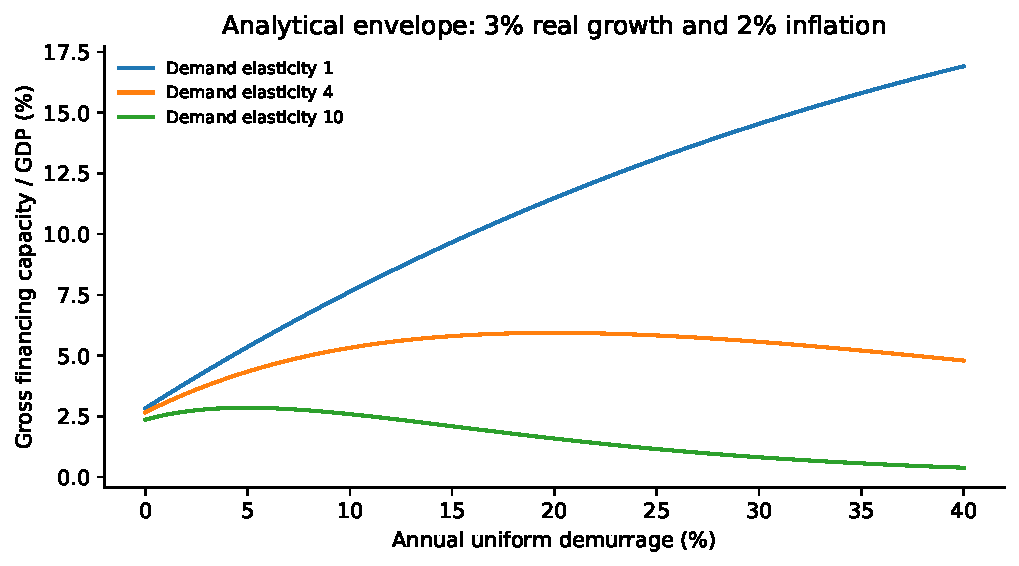
\includegraphics[width=.92\linewidth]{figures/frontier.pdf}
\caption{Analytical gross financing envelope with endogenous money demand. Values are assumed scenarios, not observed national revenue capacities. The holding levy is part of the resource transfer.}
\end{figure}


\section{What can ownership add to regulation and fiscal redistribution?}
\subsection{The unit of comparison is a policy contract}
A legally required grant of new equity changes private property claims. Calling it usownership does not remove its distributive incidence. Conversely, legislation can create property rights, and a tax-financed asset grant changes a household's balance sheet. The useful distinction is between contracts that distribute current income, accumulate enforceable claims, influence production or insure risks. Each can be implemented through legislation, private agreements or combinations of the two.

Consider five comparators. A conventional transfer supplies current spending power and insurance. A capital-income tax shifts part of the financing away from wages. A dividend levy can be earmarked to the very participants who would receive equity. A tax-funded asset grant or subsidy-for-equity arrangement can build legal ownership. Competition, labour and data regulation change rents, bargaining positions and admissible conduct. No single one is an adequate substitute for every function of the others. An ownership requirement does not enforce product safety, and a public income floor does not eliminate monopoly power.

\subsection{A cash-flow equivalence benchmark}
Let $o_{ij}$ denote household $i$'s original ownership fraction of firm $j$, with no subsequent private share trades. Let $U_{j,t}$ be aggregate user equity under \eqref{eq:U}, $u_{ij,t}$ its household allocation, and $\Pi_{j,t}$ the firm's distributable cash. Legacy holdings then equal $(1-U_{j,t})o_{ij}$. The equity system pays
\begin{equation}
D^E_{i,t}=\sum_j\big[(1-U_{j,t})o_{ij}+u_{ij,t}\big]\Pi_{j,t}.\label{eq:equitypayout}
\end{equation}

\begin{proposition}[Matched dividend-levy equivalence]\label{prop:equivalence}
Suppose profits, investment, participant weights, subsequent taxes and information are identical, the levy is enforceable, and shares are not traded. Retain original legal ownership, levy $U_{j,t}$ of firm $j$'s distributable cash pro rata from original holders, and rebate $u_{ij,t}\Pi_{j,t}$ to participant $i$. This system reproduces \eqref{eq:equitypayout} in every period and state. In a model where household decisions depend only on those cash flows and opening cash, both systems generate identical consumption, MVI, money and prices.
\end{proposition}
\begin{proof}
Original-holder income after the levy is $\sum_j(1-U_{j,t})o_{ij}\Pi_{j,t}$. Adding the rebate gives \eqref{eq:equitypayout}. Given equal initial cash, the next cash balance and all income-dependent decisions coincide. Induction establishes the path result. This argument holds conditional on identical investment; it does not assume that a real tax and a real equity contract necessarily induce identical behaviour.
\end{proof}

The proposition is an intentionally demanding null benchmark. The simulations implement the levy through a \emph{shadow entitlement register}, using the same contribution history, dilution schedule and investment wedge as usownership. The gross earmarked levy equals its rebate; it is reported separately from conventional tax revenue and MVI. It is not fictitious additional seigniorage. The comparator is sophisticated rather than a description of a current tax system. Its purpose is to show what an equity label alone cannot establish.

The same result qualifies the stock-versus-flow argument. If identical future tax liabilities and benefit claims are enforceable and capitalised at the same state-contingent discount factors, economic net wealth is also identical. A lower Gini of \emph{legal book assets}, which omits those future fiscal claims, is not by itself a welfare gain. Legal ownership can still matter for votes, sale, collateral, inheritance and protection against policy revision. These are additional contractual rights, not new real output created by distributing certificates.

\subsection{Gradual does not mean inexpensive}
At fixed firm value, a grant of $\delta$ new shares per old share transfers $\delta/(1+\delta)$ of the post-issue claim. At constant annual issuance of 0.5\%, 1\% or 2\%, user shares after 50 years are respectively 22.1\%, 39.2\% and 62.8\%. The small yearly rate is politically and operationally different from an immediate large transfer, but its compound incidence is not small.

For a transparent valuation calculation, let total end-year dividends grow at $g_D$ and let investors discount at $r>g_D$. The ratio of legacy-share present value with perpetual constant dilution to its no-dilution value is
\begin{equation}
\frac{V_\delta}{V_0}=\frac{(1+r)-(1+g_D)}{(1+r)(1+\delta)-(1+g_D)}.\label{eq:pv}
\end{equation}
This follows by summing two geometric series with ratios $(1+g_D)/(1+r)$ and $(1+g_D)/[(1+r)(1+\delta)]$. With the illustrative assumptions $r=8\%$ and $g_D=3\%$, the legacy-value losses are 9.7\%, 17.8\% and 30.2\% at the three issuance rates. These are mechanical perpetuity values, not estimated financing-cost effects. The same burden arises under a fully anticipated matched levy.

At a particular horizon, retaining the old shareholders' terminal wealth requires total company value to rise by $1/(1-U_T)-1$ relative to the no-grant counterfactual. Thus 1\% annual issuance over 50 years would require about 64.5\% additional total value to offset its ownership dilution. It would be unjustified to assume that stronger engagement automatically supplies this gain. Supplementary Table S1 reports the complete incidence arithmetic.

\subsection{Conditional advantages worth testing}
Four margins are promising. \emph{First, persistent claims}: a vested share may survive the expiry of a programme's new-award budget. A durable entitlement can reduce renegotiation and help participants plan long-term investment in an ecosystem. A legally protected tax-funded endowment may do the same; corporate rights are themselves vulnerable to insolvency, recapitalisation and changes in law. The relative security of the two contracts must be measured.

\emph{Second, participation and governance}: a participant who contributes expertise, useful feedback or productive complements can share a firm's residual upside and, where rights permit, its governance. That may reward contributions inadequately covered by conventional employment or purchase contracts. Fixed participation scores in our macro model do not estimate the resulting effort response. Non-voting shares should not be presented as democratic control, and fragmented minority positions may require representation to exercise any practical influence.

\emph{Third, issuance-date liquidity}: a new-share grant need not require a firm or government to pay cash at the issue date. Compared with a cash-financed share purchase, it can be useful where liquidity is scarce even though its economic cost falls on existing holders. It can also attach claims before profits are distributed. Whether a cash-flow tax with loss offsets, deferred payments or equity settlement is equally effective remains a counterfactual, not an impossibility.

\emph{Fourth, a verifiable accumulating claim}: a disclosed share fraction and register can make the allocation rule inspectable and avoid repeatedly determining an unlisted firm's market value merely to compute the number of shares. That does not remove valuation from accounting, tax or disputes. Contribution verification, group consolidation, corporate actions, buybacks and anti-dilution protection create their own administrative burdens. No percentage-of-GDP bureaucracy saving is assumed.

A useful conditional test is whether the present value of additional participant value, governance gains, commitment and financing relief exceeds measurement costs, concentrated risk and investment distortions. Denote those components by $V_p,V_g,V_c,V_l$ and $C_m,C_r,C_i$. The proposal's institutional case requires
\begin{equation}
\Delta W_{\rm institutional}=V_p+V_g+V_c+V_l-C_m-C_r-C_i>0.\label{eq:wedge}
\end{equation}
Equation~\eqref{eq:wedge} organises quantities to estimate; it is not an estimated welfare equation or an assumption that the left side is positive. The frictionless replication benchmark sets the differential terms to zero. This is a stronger empirical research agenda than treating all conventional policy as incapable of accumulating assets.

\subsection{Why the Internet-of-Value paradigm changes the practical comparison}
The cash-flow equivalence proposition is deliberately technology-neutral. In a frictionless model, legal equity and a perfectly credible matched levy can deliver identical cash. The practical comparison changes when the institutional cost of maintaining those claims differs. The existing financial architecture is highly capable for large conventional securities, but repeated low-value allocations to millions of heterogeneous users are not its standard use case. A tokenised infrastructure can represent fractional claims, transfer conditions, vesting and payment instructions in the same programmable environment \citep{bis2023,bis2025}.

This produces a conditional implementation advantage rather than an economic free lunch. Under usownership, a user's verified contribution can update an accumulating property claim without the state repeatedly collecting cash and purchasing assets on the user's behalf. Dividends can be routed to the current owner, corporate actions can update the same register, and an eventual voluntary exchange into diversified assets can settle against tokenised money. Under a conventional levy, the fiscal authority can reproduce income but must maintain a separate entitlement rule and political commitment. Either architecture can be designed badly; programmability simply lowers some contracting and reconciliation frictions when assets themselves are digital and executable.

The structural-change argument is therefore stronger than a blockchain argument. As economic value migrates from documents and disconnected databases toward digitally native or tokenised claims, ownership design becomes part of the software and legal architecture through which value moves. The European Commission now describes tokenisation as a possible path toward an Internet of Value, while the BIS sees programmable money and assets as components of a next-generation monetary system \citep{eciov2026,bis2025}. Usownership is tailored to that environment because the distribution mechanism is itself a stream of small ownership events. Its comparative advantage should disappear in the model if programmable infrastructure does not reduce implementation costs or if equivalent fiscal entitlements provide the same durability and governance.

The technology also creates new failure modes. An erroneous contribution oracle can automate the wrong allocation at scale; a compromised key can transfer a legally valuable claim; privacy-invasive scoring can turn ownership into surveillance; and incompatible ledgers can recreate fragmentation. These risks belong inside the cost terms of Equation~\eqref{eq:implementation}. A public permissionless blockchain is neither necessary nor assumed.

\subsection{Monetary finance is an auxiliary bridge, not a unique bridge}
Declining labour's share can raise distributional pressures without reducing the absolute real wage bill: sufficiently rapid output growth can offset the share decline. The Commission's 2026 tax-trends update reports 2024 EU taxes at 39.4\% of GDP, of which labour taxes and social contributions provide 51.5\% \citep{taxtrends2026}. Their product is 20.29\% of GDP. At fixed GDP, rates and composition, a 25\% or 50\% contraction in this base would reduce receipts by 5.07 or 10.15 percentage points of GDP. These are static exposures, not forecasts; neither job exposure nor a falling labour share implies either contraction.

A government can bridge an income disruption with redesigned taxes, debt, existing reserves, public asset income or seigniorage. Borrowing may be especially relevant to a temporary shock. Because the laboratory excludes sovereign debt, it cannot establish a timing advantage of monetary finance over debt-financed transfers. The useful monetary question is more limited: how much financing can coexist with sustained transaction demand and acceptable prices, after accounting for the incidence of any holding levy? The monetary accounting in the following section gives a bounded answer rather than an instruction to replace fiscal policy with a programmable ledger.

\section{Model, experiments and identification}
\subsection{A deliberately bounded transition laboratory}
The simulation contains 400 equally weighted synthetic resident-equivalent households and three representative firm types with output weights $(0.35,0.35,0.30)$. Initial GDP and prices equal one; capital/output is three and money/output is 0.6. Wage and initial equity allocations are heterogeneous correlated draws. There is no estimated household survey, endogenous entry, banking sector, debt market or foreign sector. All payment balances are direct sovereign liabilities; productive capital is financed through retained earnings. The model is stock-flow consistent within this boundary, not a full account of the transition from present banking arrangements.

A normalised logistic automation path $a_{j,t}$ starts at zero and differs by activity. Labour's gross-output share is $\lambda_{j,t}=0.10+0.48(1-a_{j,t})$. Gross investment shares are
\begin{equation}
\nu_{j,t}=\operatorname{clip}\{0.22+0.025a_{j,t}-\chi\delta_{j,t},0.04,0.40\},\quad\chi=0.60,
\end{equation}
subject to a positive dividend residual $1-\lambda_{j,t}-\nu_{j,t}$. The cost parameter $\chi$ is assumed and stressed, not estimated. The matched-levy comparator deliberately uses the same investment wedge. This isolates the legal form of the payout; it does not predict actual tax-versus-dilution investment responses.

Capital evolves as $K_{j,t+1}=0.94K_{j,t}+\omega_j\nu_{j,t}Y_t$. Raw potential output and the resource ceiling are
\begin{equation}
Y_t^{\rm raw}=\sum_j\omega_j(1.01)^t\exp(\gamma a_{j,t})\left(\frac{K_{j,t}}{K_{j,0}}\right)^{0.4},\quad R_t=\frac{1.30(1.035)^t}{1+0.15\bar a_t}.
\end{equation}
Potential output is the smaller of these quantities. The ceiling is an assumed resource constraint, not an observed energy price or engineering frontier. A temporary supply shock and alternative resource-growth rates test its influence. Normalised heterogeneous task exposure allocates the wage bill. The reported labour-demand proxy is not a national unemployment estimate.

\subsection{Cash, spending, fiscal closure and prices}
Let $x_{i,t-1}$ denote opening nominal cash, $\ell_{i,t}$ the household holding levy, $h_{i,t}$ its transfer and $r_{i,t}$ its share of current factor cash income, with $\sum_i r_{i,t}=1-\nu_t$. In the baseline, net factor share is $\widetilde r_{i,t}=(1-\tau_t)r_{i,t}$. The capital-focused tax benchmark instead uses
\begin{equation}
\widetilde r_{i,t}=(1-\tau^w_t)r^w_{i,t}+(1-\tau^k_t)r^k_{i,t},\quad
\tau^w_t=\min(0.6\tau_t,0.95),\quad\tau^k_t=\min(1.4\tau_t,0.95).
\end{equation}
The multipliers define an illustrative rebalancing, not an optimal schedule. Both rates and the transfer rule are solved within the same nominal closure, and capital taxes are imposed on distributed cash income rather than assumed to apply to the entire stock.

Households spend $C_{i,t}=\alpha_{i,t}[x_{i,t-1}-\ell_{i,t}+\widetilde r_{i,t}N_t+h_{i,t}]$, retaining the rest as cash. Here $\alpha_{i,t}=1/(1+\kappa_{i,t})$. Desired liquidity $\kappa$ responds negatively to expected inflation relative to target, the effective levy and the return advantage of alternative assets. The central elasticity is four; expectations adjust at 0.3. This is a behavioural closure rather than a utility-maximising portfolio model. Portfolio substitution changes spending and the demand for balances; there is no simulated offshore asset stock.

For given taxes and transfers, nominal expenditure is solved exactly:
\begin{equation}
N_t=\frac{\sum_i\alpha_{i,t}(x_{i,t-1}-\ell_{i,t}+h_{i,t})+G_t}
{1-\nu_t-\sum_i\alpha_{i,t}\widetilde r_{i,t}}.\label{eq:closuremain}
\end{equation}
This is the joint goods/cash accounting solution, not an assumed Keynesian multiplier. With potential output $Y_t^*$, prices satisfy $P_t=\max\{N_t/Y_t^*,0.98P_{t-1}\}$ and output is $N_t/P_t$. Excess demand raises prices; weak demand may lower utilisation when downward price adjustment is constrained. There are no endogenous relative prices or an estimated Phillips curve.

Public purchases equal 22\% of forecast nominal capacity. The reference income floor is 25\% of forecast potential GDP per resident-equivalent unit. Universal payments are calibrated to predicted after-tax income at the tenth percentile; targeted payments fill each predicted gap. They are different transfer designs, not identical coverage rules. Forecast errors, taxes and the holding levy can leave realised shortfalls, which are reported separately.

The adaptive monetary rule targets money growth based on forecast capacity growth, changes in desired liquidity and the previous inflation gap. A bounded scalar root chooses a conventional tax parameter in $[0,0.85]$ to attain that money stock. The maximum is a computational policy bound, not a claim of political feasibility. Fixed-tax variants instead allow issuance to close the budget. Thus near-target inflation in the adaptive cases can require substantial residual taxation; it is not imposed proof of successful seigniorage-only financing. The supplement gives the full timing, equations and parameters.

\subsection{Experiments and diagnostic outcomes}
The inherited design contains ten policies across slow, medium and fast automation, 36 robustness experiments and 128 common Latin-hypercube configurations across three paired policies: 450 runs. The additional comparison executes nine policies across the three automation paths and six policies across twelve robustness configurations: 99 runs. There are \emph{549 executed macro paths in total}, including repeated control configurations and explicitly failed paths, not 549 independent empirical observations. We report main counterfactuals at 50 years and retain 10-, 25- and 100-year original scenarios in the supplement and data. Century-scale extensions hold agents and firm types fixed and are not forecasts.

B0 provides targeted protection; B2 a universal transfer; B5 adds usownership; B6 adds the holding-levy monetary architecture; B7 allocates firm equity equally rather than by contribution. B10 adds capital-focused taxation without user equity. B11 matches B5's dividends through a levy and rebate; B12 matches B6. B13 combines usownership and the monetary architecture with targeted income protection. All have the same production opportunities, initial household draws and stated public-service commitment within a scenario. No baseline is described as a fully calibrated current tax system.

The slow, medium and fast logistic midpoints are 40, 20 and 10 years; speeds are 0.08, 0.14 and 0.30; saturation values are 0.65, 0.90 and 0.98. Productivity-gain coefficients are 0.35, 0.90 and 1.60. The design spans hypotheses rather than assigns their probabilities. Robustness changes money demand, public purchases, income-floor indexation, score integrity, contributor coverage, dilution speed, investment response and resource limits.

Outputs distinguish MVI, participant dividends or rebates, conventional taxes, pass-through levies, monetary financing, money balances, coverage, consumption and legal book wealth. Book wealth is money plus corporate book equity; it omits housing, pensions and capitalised fiscal claims. Mean log consumption omits leisure, risk and public-service utility and is not a complete welfare criterion. A narrow sunset diagnostic requires MVI below 1\% of GDP for the last five years of a 50-year run, independently of adequacy. Price-band success requires absolute inflation at most 5\% throughout. Every period checks monetary and goods identities and equity conservation. The extended suite also verifies the exact cash-flow replication and rejects incompatible secondary sales in that experiment.

\section{Results: ownership, income protection and financing are different margins}
\subsection{What changes when the counterfactual is strengthened?}
Table~\ref{tab:comparison} summarises the new 50-year medium-automation comparison. The values describe a synthetic scenario. Equal starting conditions permit controlled comparison, but the behavioural equations and policy functions are not empirically identified.

\begin{table}[htbp]\centering\small
\caption{Medium automation, model year 50: strengthened policy comparisons}\label{tab:comparison}
\begin{tabular}{@{}lrrrrr@{}}
\toprule
Policy & $Y_{50}$ & MVI/GDP & Tax/GDP & Participant/GDP & Book Gini \\
\midrule
B0 & 6.48 & 7.07 & 25.01 & 0.00 & 0.768 \\
B2 & 6.48 & 19.03 & 37.04 & 0.00 & 0.754 \\
B5 & 6.48 & 10.57 & 28.53 & 17.14 & 0.583 \\
B6 & 6.48 & 10.16 & 27.13 & 17.14 & 0.584 \\
B7 & 6.48 & 5.96 & 23.91 & 17.14 & 0.560 \\
B10 & 6.48 & 16.98 & 34.98 & 0.00 & 0.749 \\
B11 & 6.48 & 10.57 & 28.53 & 17.14 & 0.745 \\
B12 & 6.48 & 10.16 & 27.13 & 17.14 & 0.749 \\
B13 & 6.48 & 1.91 & 18.75 & 17.14 & 0.595 \\
\bottomrule
\end{tabular}

\par\smallskip\footnotesize Flow columns are percentages of GDP. B0: targeted transfers; B2: universal transfers; B5: user equity; B6: user equity plus monetary levy; B7: equal equity; B10: capital-focused tax; B11/B12: matched levies for B5/B6; B13: targeted hybrid. Tax/GDP excludes earmarked participant pass-through levies, which equal 17.14\% of GDP in B11/B12. Book Gini excludes capitalised future fiscal claims.
\end{table}

Relative to B2, adding user equity in B5 reduces MVI by 8.46 percentage points of GDP, from 19.03\% to 10.57\%. Adding the monetary holding-levy architecture in B6 contributes a further 0.41 percentage points, bringing MVI to 10.16\%. Approximately 95\% of the combined transfer reduction along this sequential comparison precedes the special levy. This is an order-dependent ablation, not a structural attribution or a Shapley decomposition. B5's book-wealth Gini of 0.583 is marginally lower than B6's 0.584; the monetary instrument is not unambiguously more equalising.

The stronger tax comparator B10 reduces MVI to 16.98\% and conventional tax/GDP to 34.98\%, compared with 19.03\% and 37.04\% in B2. Thus adapting tax incidence helps even without equity grants. The experiment does not search the space of optimal nonlinear taxes, capital-income smoothing or behavioural responses. It supports a comparison against this explicit schedule, not a conclusion that usownership dominates the best possible fiscal system.

Targeting is at least as consequential. B0 requires MVI of 7.07\% of GDP, below the 10.16\% universal hybrid. Combining targeted protection with usownership and the levy in B13 lowers it to 1.91\%, with residual conventional taxation of 18.75\%. Universal and targeted schemes share a reference floor but not the same coverage, information requirements or political contract. Predicted-gap targeting remains imperfect in realised outcomes. The result is therefore a strong reason to separate protection policy from ownership policy, not a proof that means testing is always preferable.

\begin{figure}[htbp]\centering
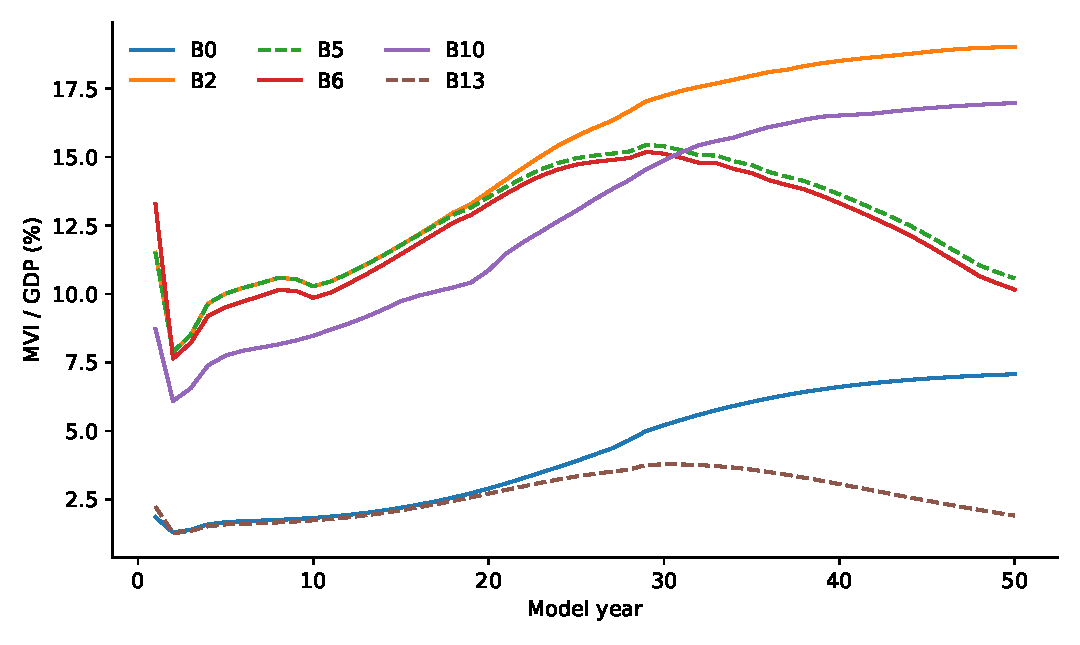
\includegraphics[width=.90\linewidth]{figures/comparative_transfer.pdf}
\caption{MVI paths under strengthened counterfactuals. Targeting and ownership each matter; the holding levy is a smaller incremental change in this scenario.}
\end{figure}

\subsection{The matched levy removes the claim of automatic cash-flow superiority}
B11 reproduces B5 and B12 reproduces B6 in household cash income, consumption, MVI, monetary balances, prices and output. Across three automation paths and eight recorded macro metrics for each matched pair, the maximum discrepancy is zero at the exported numerical precision. This is an implementation check of Proposition~\ref{prop:equivalence}, not an independent empirical finding.

The register reallocates 17.14\% of GDP in participant cash income at year 50 under either legal form in the medium path. In B6 this is user dividends; in B12 it is an earmarked levy rebate. Ordinary tax/GDP is 27.13\% in each. Including the gross pass-through, B12 records total taxes of 44.27\% of GDP and an equal additional rebate flow. That larger gross tax number does \emph{not} establish a larger net resource burden or lower efficiency. It is the cash-flow analogue of the in-kind equity redistribution.

Legal book ownership does differ: user equity is 29.67\% in B6 and zero in B12. Their book-wealth Ginis are 0.584 and 0.749. Because future tax and rebate claims are not included in that measure, it cannot adjudicate their economic net wealth or welfare. An equal-payoff valuation would capitalise both the legacy owners' levy liability and the participants' rebate asset. The genuine remaining research questions concern enforceability, control, transferability, risk and participation responses. They are not solved by the wealth-accounting label.

\begin{figure}[htbp]\centering
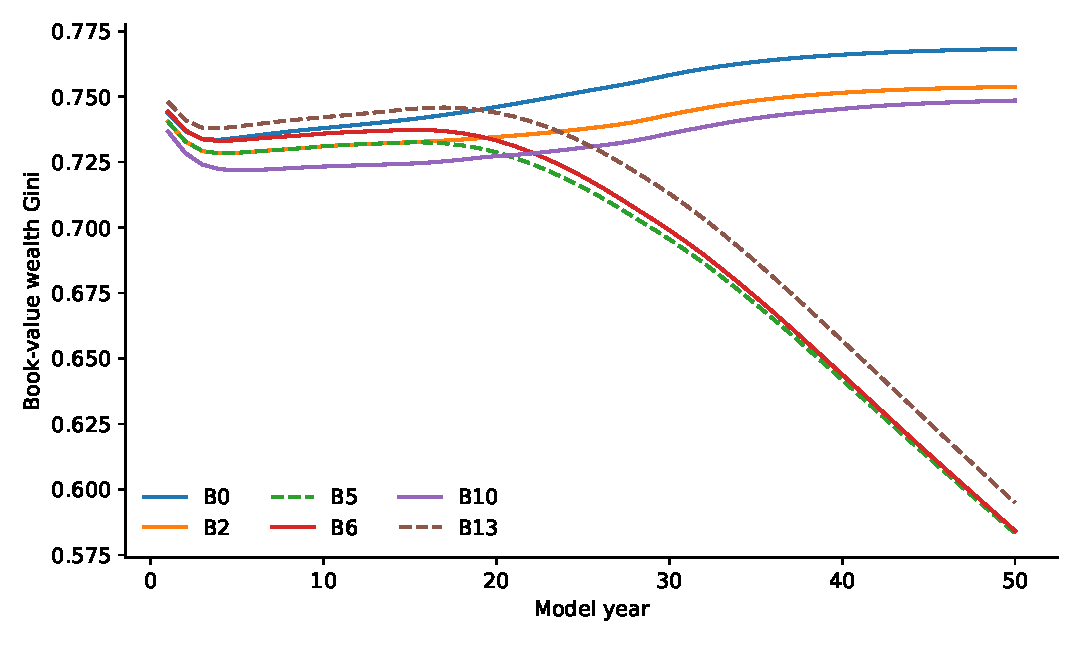
\includegraphics[width=.90\linewidth]{figures/comparative_ownership.pdf}
\caption{Legal book-wealth concentration. These series exclude capitalised fiscal claims and must not be read as welfare rankings over matched income streams.}
\end{figure}

\subsection{The financing limit remains binding}
The central B6 hybrid uses conventional taxes of 27.13\% of GDP at year 50. Fiscal issuance before the holding levy is 4.60\% of GDP: 1.31 percentage points correspond to the explicit levy and 3.29 to net monetary financing. Near-target inflation, peaking around 2.13\% over the 50-year path, is conditional on the residual-tax instrument and the price closure.

Fixed-tax monetary financing performs very differently. In the original medium path, B3 reaches roughly 40.3\% peak inflation; adding demurrage in B4 raises that peak to roughly 45.1\%. The induced reduction in desired balances can outweigh part of the mechanical cancellation effect. These are model-specific counterexamples, not predictions that negative interest is always inflationary. The central no-conventional-tax case fails numerically before substantial ownership diffusion. Extreme rates near the numerical stop are diagnostics, not quantitative hyperinflation forecasts.

A narrower no-tax case retains the original proposal's 7\% public-purchases block, sets the income reference to 15\% and initial money/GDP to one. It survives 50 years and eventually has no top-up, but peak inflation is about 7.03\%, outside the strict 5\% band. It does not maintain the central public-service commitment or the 2\% target. This favourable counterexample is retained because the relevant object is a feasible financing region, not an unconditional impossibility claim. Higher money demand is an assumption, not a policy instrument that can simply be ordered into existence.

\begin{figure}[htbp]\centering
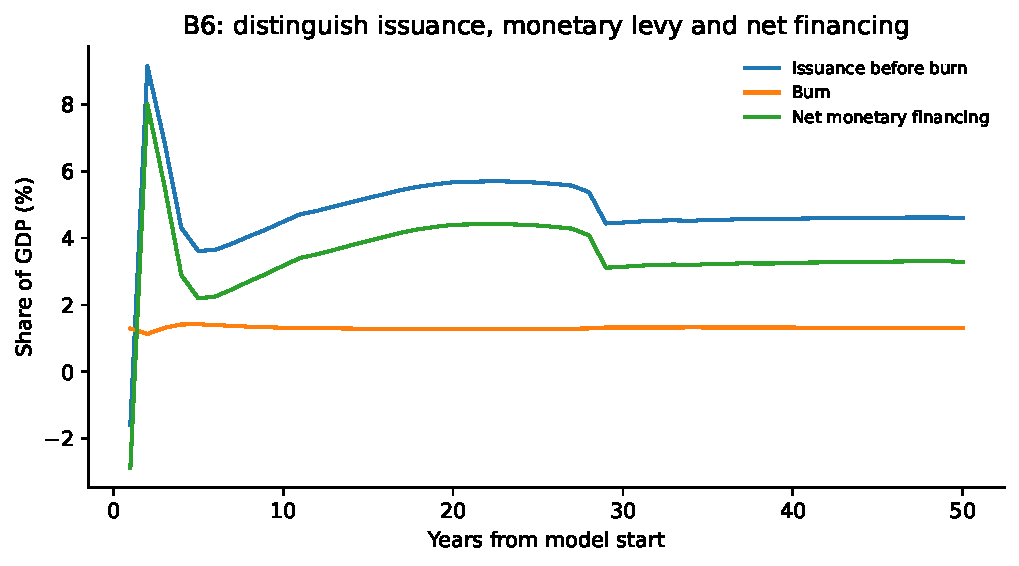
\includegraphics[width=.90\linewidth]{figures/monetary_flows.pdf}
\caption{Money financing in the medium hybrid. Issuance before the holding levy must not be added to that levy as though both were independent free resources.}
\end{figure}

\subsection{Coverage and the speed of the ownership bridge}
The original medium hybrid's MVI/GDP peaks near 15.19\% in year 29, then falls to 10.16\% in year 50. It does not disappear within that window. Only six of the 128 original hybrid parameter configurations meet the specified five-year sunset criterion; the corresponding counts are four for B5 and zero for B2. These frequencies describe the chosen parameter box, not probabilities of real-world success. A prosperity-indexed floor is harder to replace than a fixed-real floor because growing output also raises the income objective.

The participant selection mechanism is crucial. Excluding the lowest-initial-wage 20\% from equity grants leaves aggregate user ownership unchanged but raises MVI to about 19.15\% of GDP at year 50. Large aggregate capital claims do not help a person who does not receive them. The equal-grant B7 comparator lowers MVI to 5.96\% and the book Gini to 0.560, outperforming contribution weighting on these distributional metrics. Since contribution-related effort gains are not estimated, there is no basis for treating this as an inferior policy. It is a transparent trade-off between the participation rationale and broad coverage, not an instruction to replace the user's firm-specific design with a pooled fund.

Consumption-only allocation, score capture and early sales weaken the ownership result in the inherited robustness runs. Immediate permitted liquidation leaves user equity around 7.72\% and a book Gini near 0.753; ten-year vesting with a retained core moderates that channel. However, restrictions cost liquidity and diversification. People facing disability, care obligations or poor digital access must not be required to supply behavioural data merely to obtain subsistence support. The MVI floor and participant equity remain separate entitlements.

\subsection{Output and investment are not free gains}
Several medium-automation cases reach exactly the same year-50 real output, 6.481 times the initial index. The resource ceiling binds. This is not evidence that equity diffusion is costless, nor that any policy generates a growth dividend. In the original unconstrained-resource sensitivity, output at year 50 is about 6.862 with no dilution-investment penalty, 6.738 with the central penalty and 6.227 with a higher penalty. Their differences are consequences of assumed investment responses, not empirical elasticity estimates.

The additional 72 robustness paths compare the strongest practical benchmarks under twelve common parameter settings. They retain adverse cases, rather than selecting only a favourable equity path. The full machine-readable results include coverage gaps, residual taxation and the log-consumption diagnostic as well as wealth. No welfare-superiority claim is based on a single Gini or on nominal GDP growth. The unresolved investment, governance and participation responses are precisely the parameters needed for an empirical test of the institutional advantage in \eqref{eq:wedge}.

\section{Institutional design, implementation and empirical priorities}
\subsection{An ownership contract, not a substitute for the state}
An implementable usownership contract must specify the entity whose equity is allocated, eligible persons, the issue schedule, the unit of contribution, vesting, cash distributions, voting rights and treatment of corporate actions. Shares should attach to the consolidated source of surplus rather than a shell subsidiary from which royalties and valuable assets can be removed. Mergers, buybacks, private recapitalisations and offshore restructurings need explicit rules. Those issues are shared with in-kind equity taxation, not eliminated by a token register.

A consumer, safety evaluator and plugin creator can have different legitimate claims. The score must nevertheless distinguish customer use from paid labour, pre-existing intellectual property and personal-data consent. The baseline's concavity in expenditure limits the advantage of wealthy consumers but does not establish an optimal distribution. Raw attention time should not be an uncapped reward base. Productive evaluations should be audited against outcomes where possible, and appealable decisions should not depend solely on an opaque AI classifier. Sybil resistance, proportional audits and exclusion safeguards are implementation costs to measure, not decorative technical features.

The minimum architecture could be a regulated digital share register with conventional payment accounts and auditable aggregate issuance; a stronger Internet-of-Value architecture would place tokenised claims and programmable settlement on interoperable rails. Distributed ledgers may assist coordination across independent institutions; privacy-preserving proofs may verify an allocation computation without publishing raw behavioural histories. Neither verifies that the underlying contribution data are true. Full public transaction histories are not required and would create disproportionate privacy risks. AI is appropriate for decision support and error detection, not unreviewable monetary or property-right decisions.

\subsection{Money, public services and the European boundary}
The sovereign-money assumption is economically consequential. Moving commercial deposits into sovereign accounts requires a bank-funding and legacy-debt transition; it does not give the government a free claim equal to all existing broad money. Foreign-currency substitution and exchange-rate pressure may make money demand more elastic than in this closed model. A legal ban on other payment instruments does not eliminate alternative stores of value.

For Europe, economic feasibility in a hypothetical sovereign system must be distinguished from present law. Article 123 TFEU restricts central-bank financing of public authorities \citep{tfeu123}. The digital-euro work is not an existing mandate for the programmable demurrage and fiscal financing assumed here \citep{ecbpilot2026,bundesbank2026}. The manuscript therefore proposes neither unilateral national euro issuance nor an assertion that the full architecture can be implemented under current treaties. A legal evaluation of mandatory share issuance, corporate governance, securities, data protection and cross-border capital movements is required in parallel with economic validation.

Public provision must remain explicit. A 7\% public-services case and the 22\% services block in the central model represent different commitments; neither equals the total observed general-government budget, which includes transfers and other items. Moving healthcare or pensions to private expenditure is not an administrative saving. No large bureaucracy saving, subsidy multiplier or automatic tax-compliance advantage is imported from the original exploratory calculations.

\subsection{A staged research and implementation path}
The participant-equity contract can be tested before monetary-regime replacement. A first empirical design would compare actual equity awards with present-value-matched cash rewards, plus a cash reward that accumulates into a financial asset. These arms distinguish incentives from simple payment size and distinguish user equity from asset ownership more generally. Matched eligibility, contribution tasks and transparent consent should be held fixed. Relevant outcomes include productive feedback quality, retention, additional sales, owner returns, participation exclusion, administration cost and portfolio concentration. Attrition and non-participation must be reported, not discarded.

A second stage would estimate how the award schedule affects entry, finance and investment. Both dilution and a matched levy should face common demand shocks and an explicit commitment environment. A third stage would link those estimates to household survey data and a bank/debt/external-sector model. Only then could the monetary bridge be evaluated against debt finance and conventional fiscal adjustment on a comparable macroeconomic basis. This sequencing tests the most distinctive institutional component without requiring a sovereign currency reform to learn whether participants value equity.

A much-later diversification path can preserve the initial design: firm-specific claims, vested portability, voluntary exchange into diversified assets and only subsequently possible sectoral or public pools. A century is an illustrative scenario horizon, not a prescribed institutional timetable. Even within an extended firm-specific phase, households need access to risk management; preserving the participation principle does not require exposing them permanently to one firm's bankruptcy.

\subsection{Novelty, feasibility and the 2027--2037 opportunity window}
The novelty is best stated as an integration across an identifiable research lineage rather than as a claim that every ingredient is new. De la Rosa Esteva's 2022 IoV chapter anticipated a ``Value Deluge'' associated with the large-scale migration of value onto ledgers and linked interoperable IoV infrastructure to the democratisation of finance and property \citep{delarosa2022iov}. ERC-4950, created the same year, explicitly introduced ``Usowners'' as users who can become partial NFT owners and proposed entangled tokens as a linked-control primitive \citep{erc4950}. The present paper adds the missing generalisation: usownership is a recurring firm-level institution with heterogeneous contribution weights, exact dilution accounting, automation-linked accumulation, coverage constraints, fiscal replication tests and a bounded monetary bridge. The contribution is therefore not the first use of partial user ownership; it is the structural-transition model that connects an ownership primitive to the changing distribution of production income.

Feasibility has three distinct layers. Technically, the enabling environment is materially closer than it was in 2022. The ECB reports that European issuers had placed close to EUR~4 billion of DLT-based fixed-income instruments since 2021 and that Eurosystem exploratory work processed roughly EUR~1.6 billion across nine jurisdictions \citep{cipollone2026}. BIS work in 2026 similarly treats tokenisation and trusted programmable money as a plausible next-generation financial architecture rather than as a purely crypto-native experiment \citep{bis2026}. Institutionally, however, tokenised shares remain shares: corporate, securities, competition, privacy and insolvency law continue to govern the claim. Economically, the present simulations show that neither dilution nor monetary finance is free. A pilot can therefore be technologically feasible well before a mandatory national regime is economically or legally justified.

The next decade is relevant because the ownership mechanism is intentionally gradual. At a constant 1\% annual new-share issue, Proposition~\ref{prop:accumulation} implies that users collectively reach only about 9.5\% ownership after ten years; at 2\%, the corresponding share is about 18.0\%. A mechanism intended to cushion a future ownership gap cannot be designed only after that gap has become acute. At the same time, present evidence does not justify treating radical automation by 2037 as certain. \citet{katz2026} estimate modest realised aggregate GDP effects from generative AI through 2025, whereas \citet{fannguyen2026} value observed AI-enabled time savings at a labour-cost equivalent of USD~2.7 trillion, or 3.4\% of GDP, and transformative-AI models permit much larger factor-distribution changes under stronger assumptions \citep{trammell2026}. The 2027--2037 period is therefore best understood as an \emph{institution-design window under deep uncertainty}: production technology and financial rails are both changing, while ownership institutions can be tested before path dependence and concentration become harder to reverse.

\begin{table}[htbp]\centering\small
\caption{Illustrative evidence-gated path for the next decade; dates are design horizons, not forecasts}
\begin{tabularx}{\linewidth}{@{}p{.16\linewidth}p{.27\linewidth}p{.31\linewidth}X@{}}
\toprule
Illustrative horizon & Usownership institution & Programmable-value infrastructure & Evidence gate before scaling \\
\midrule
2027--2030 & Voluntary or contract-based firm pilots; matched equity/cash experiments; vesting and retained-core tests & Regulated digital share registers or tokenised securities; auditable contribution records & Participation coverage, investor response, administration cost, score manipulation and legal treatment \\
2031--2033 & Interoperable firm-specific awards; portability and diversification options; stronger anti-reconcentration rules & Common token/registry standards, automated corporate actions and conditional settlement & Demonstrated net operating-cost advantage and acceptable privacy, oracle, cyber and market-liquidity risks \\
2034--2037 & Conditional wider adoption in sectors where automation materially shifts factor income & Integration with trusted tokenised money or central-bank settlement where legally available & Measured labour-share/displacement effects, money demand, inflation headroom and evidence that ownership income reduces transfer needs \\
\bottomrule
\end{tabularx}

\end{table}

The paper deliberately keeps two time horizons distinct. The first is the 2027--2037 institutional window, in which firm-level pilots, contribution measurement, legal design and programmable-value rails can be tested before any economy-wide adoption. The second is a 50-year structural horizon, illustratively 2027--2077, used to study the cumulative ownership transition rather than to date a forecast. The distinction matters because compounding is slow: absent sales and other issuance, a constant 1\% annual issue produces about 9.5\% user ownership after ten years but about 39.2\% after fifty years. Model year 50 therefore remains the principal long-run comparison for whether usownership can become a material source of household capital income and reduce reliance on MVI and monetary finance; the 100-year extension is retained only as a more remote sensitivity exercise.

\section{Limitations and conclusion}
The main unestimated components are the productivity and investment responses to ownership, the causal value and cost of contribution measurement, relative institutional durability, corporate decision rights, and monetary demand after regime change. The model omits bank credit, sovereign debt, trade, market equity prices, endogenous corporate entry and generational renewal. Its declining wage share and resource ceiling are assumed. These omissions are not minor uncertainty intervals around a forecast; they define the domain of the experiment.

The revised comparison supports a specific novelty claim. Earlier work in this research trajectory had already anticipated the migration of value onto ledgers and the need to preserve ownership across an Internet of Value \citep{delarosa2022iov}; ERC-4950 had already named ``Usowners'' and demonstrated a digital partial-ownership primitive \citep{erc4950}. This paper does not relabel those precursors as new. It generalises them into a macroeconomic institution and subjects that institution to tests absent from the precursors: heterogeneous contribution weights, exact corporate dilution, investor cost, exclusion and reconcentration, matched dividend-levy replication, stock-flow-consistent monetary accounting and transition scenarios. The strongest contribution is thus a bridge between the economics of structural change and a programmable property-rights architecture: an attempt to make redistribution increasingly \emph{pre-distributive}, by changing who accumulates productive claims before profits have to be repeatedly taxed and transferred.

Feasibility is correspondingly conditional but increasingly concrete. The simulations show that gradual participation equity can diffuse legal ownership and reduce future transfer requirements under the stated allocation and payout rules; most of the central hybrid's transfer reduction arises from ownership diffusion rather than the holding-levy monetary layer. A matched dividend levy can reproduce the same cash income under replication assumptions, so the case for usownership must rest on what the legal asset changes: durable claims, cumulative wealth, governance, participation incentives, portability and the possibility that future distributions occur without a fresh fiscal appropriation. Programmable value infrastructure can make recurring fractional awards, vesting and settlement cheaper to execute at scale, and European tokenised-market experiments demonstrate that relevant rails are no longer hypothetical \citep{cipollone2026,eciov2026,bis2026}. Yet technology does not remove dilution, securities law, contributor-verification costs or portfolio risk. The most credible near-term implementation is therefore staged and evidence-gated rather than an immediate economy-wide mandate.

The strategic opportunity lies in timing. If AI and robotics profoundly alter production during 2027--2037, waiting for labour income to collapse before building alternative ownership channels would leave policy dependent on ex post taxation and transfers precisely when the labour tax base may be weakening. If the transition is slower, early pilots still generate evidence at limited macroeconomic cost. Because usownership accumulates gradually, the institution has option value when started early: it can remain small if displacement is modest and scale only if automation materially shifts factor income. The same logic confines seigniorage to a supporting role. Bounded monetary finance can bridge part of the interval before distributed capital income matures, but money demand, inflation, real supply and public commitments remain binding constraints. The paper therefore proposes neither a taxless theorem nor a prediction of a post-work economy. It identifies a feasible research programme for 2027--2037: test whether an Internet-of-Value infrastructure can convert measured participation into durable productive ownership quickly enough to reduce the social cost of a potentially radical AI production transition, while preserving innovation, universal protection and monetary stability. The accompanying 50-year horizon, illustratively extending to 2077, asks the different structural question of whether those initially small ownership flows can compound into a sufficiently broad capital-income base to reduce MVI and seigniorage dependence over a generation-scale transition.

\section*{Data, code and generative-AI disclosure}
All simulated observations are synthetic and reproducible from the accompanying source, configurations and fixed seeds. Official aggregate anchors are separately labelled. The code, tables and figures accompany the manuscript; a public archive identifier has not yet been registered. Generative-AI assistance through ChatGPT (OpenAI) was used for literature discovery, formalisation, code development, computational checks and drafting. Reported numerical results were obtained by executing the supplied Python code; plots were generated from those results, not by synthetic-image generation. Authorship, accountability and approval belong to the submitting human authors. Funding, competing interests and author contributions are provided separately after author confirmation.

\clearpage
\bibliographystyle{plainnat}
\bibliography{bibliography}
\end{document}

